\chapter{More on certificate authentication}
\index{Certificate authentication}
\label{certificate}

\section{The X.509\index{X.509 certificates} trust model}
\label{x509:trust}

The X.509 protocols rely on a hierarchical trust model. In this trust model
Certification Authorities (CAs) are used to certify entities.
Usually more than one certification authorities exist, and certification
authorities may certify other authorities to issue certificates as well,
following a hierarchical model. 

\begin{figure}[tbp]
\caption{X.509 certification}
\includegraphics[height=9.5cm,width=7cm]{x509-1}
\label{fig:x509-1}
\end{figure}

One needs to trust one or more CAs for his secure
communications. In that case only the certificates issued by the trusted
authorities are acceptable. See figure \ref{fig:x509-1} for a typical example.
The API for handling X.509 certificates is described at section \ref{sec:x509api}
on page \pageref{sec:x509api}. Some examples are listed below.



\subsection{X.509 certificates}
An X.509 certificate usually contains information about the certificate
holder, the signer, a unique serial number, expiration dates and some other 
fields \cite{RFC3280} as shown in the table below.

\label{fig:x509}
\begin{tabular}{|l||l|}
\hline
version & the field that indicates the version of the certificate.
\\
\hline
serialNumber & this field holds a unique serial number per certificate.
\\
\hline
issuer & holds the issuer's distinguished name
\\
\hline
validity & the activation and expiration dates.
\\
\hline
subject & the subject's distinguished name of the certificate.
\\
\hline
\rowcolor[gray]{0.9}
extensions & The extensions are fields only present in version 3 certificates.
\\
\hline
\end{tabular}
\\
\\
\par
The certificate's \emph{subject or issuer name} is not just a single string. It is
a Distinguished name and in the ASN.1 notation is a sequence of several object
IDs with their corresponding values. Some of available OIDs to be used in an X.509
distinguished name are defined in \emph{gnutls/x509.h}.
\\
\\
The \emph{Version} field in a certificate has values either 1 or 3 for version 3 certificates.
Version 1 certificates do not support the extensions field so it is not possible
to distinguish a CA from a person, thus their usage should be avoided.
\\
\\
The \emph{validity} dates are there to indicate the date that the specific certificate
was activated and the date the certificate's key would be considered invalid.
\\
\\
Certificate \emph{extensions} are there to include information about the certificate's
subject that did not fit in the typical certificate fields. Those may be
e-mail addresses, flags that indicate whether the belongs to a CA etc.
All the supported X.509 version 3 extensions are shown in the table below.

\label{fig:x509_ext}
\begin{tabular}{|l|l|p{6cm}|}
\hline
subject key id & 2.5.29.14 & An identifier of the key of the subject.
\\
\hline
authority key id & 2.5.29.35 & An identifier of the authority's key used to sign the certificate.
\\
\hline
subject alternative name & 2.5.29.17 & Alternative names to subject's distinguished name.
\\
\hline
key usage & 2.5.29.15 & Constraints the key's usage of the certificate.
\\
\hline
extended key usage & 2.5.29.37 & Constraints the purpose of the certificate.
\\
\hline
basic constraints & 2.5.29.19 & Indicates whether this is a CA certificate or not.
\\
\hline
CRL distribution points & 2.5.29.31 & This extension is set by the CA, in order to inform about the issued CRLs.
\\
\hline
\end{tabular}
\\
\\
\par
In \gnutls{} the X.509 certificate structures are handled using the
\emph{gnutls\_x509\_crt} type and the corresponding private keys with
the \emph{gnutls\_x509\_privkey} type.
All the available functions for X.509 certificate handling have their 
prototypes in \emph{gnutls/x509.h}. An example program to demonstrate the 
X.509 parsing capabilities can be found at section \ref{ex:x509-info} on 
page \pageref{ex:x509-info}.

\subsection{Verifying X.509 certificate paths}
Verifying certificate\index{Verifying certificate paths} paths is important 
in X.509 authentication. For this purpose the function
\printfunc{gnutls_x509_crt_verify}{gnutls\_x509\_crt\_verify} is provided. The
output of this function is the bitwise OR of the elements of the
``gnutls\_certificate\_status'' enumeration. A detailed description of
these elements can be found in figure \ref{fig:verify}.
The function \printfunc{gnutls_certificate_verify_peers}{gnutls\_certificate\_verify\_peers}
is equivalent to the previous one, and will verify the peer's certificate in a TLS session.

\begin{figure}[hbtp]
\begin{tabular}{|l|p{7cm}|}

\hline
CERT\_INVALID & The certificate is not signed by one of the known authorities, or
the signature is invalid.
\\
\hline
CERT\_REVOKED & The certificate has been revoked.
\\
\hline
CERT\_SIGNER\_NOT\_FOUND & The certificate's issuer is not known.
\\
\hline
\end{tabular}
\caption{X.509 certificate verification}
\label{fig:verify}
\end{figure}

\par
Although the verification of a certificate path indicates that the
certificate is signed by trusted authority, does not reveal anything
about the peer's identity. It is required to verify if the certificate's
owner is the one you expect. See \cite{RFC2818} and section \ref{ex:verify-chain} 
on page \pageref{ex:verify-chain} for an example.


\subsection{PKCS \#10 certificate requests\index{Certificate requests}\index
{PKCS \#10}}
A certificate request is a structure, which
contain information about an applicant of a certificate service.
It usually contains a private key, a distinguished name and secondary
data such as a challenge password. \gnutls{} supports the requests
defined in PKCS \#10 \cite{RFC2986}. Other certificate request's format such as
PKIX's RFC2511 \cite{RFC2511} are not currently supported.

In \gnutls{} the PKCS \#10 structures are handled using the
\emph{gnutls\_x509\_crq} type. 
An example of a certificate request generation can be found at section \ref{ex:crq}
on page \pageref{ex:crq}.

\subsection{PKCS \#12 structures\index{PKCS \#12}}
A PKCS \#12 structure \cite{PKCS12} usually contains a user's private keys and
certificates. It is commonly used in browsers to export and import
the user's identities.
\par
In \gnutls{} the PKCS \#12 structures are handled using the
\emph{gnutls\_pkcs12} type. This is an abstract type that
may hold several \emph{gnutls\_pkcs12\_bag} types. The Bag types are the
holders of the actual data, which may be certificates, private
keys or encrypted data. An Bag of type encrypted should be decrypted
in order for its data to be accessed. 

An example of a PKCS \#12 structure generation can be found at section \ref{ex:pkcs12}
on page \pageref{ex:pkcs12}.

\section{The OpenPGP\index{OpenPGP!Keys} trust model}
\label{pgp:trust}

The OpenPGP key authentication relies on a distributed trust model, called
the "web of trust". The "web of trust" uses a decentralized system of 
trusted introducers, which are the same as a CA. OpenPGP allows anyone to 
sign anyone's else public key. When Alice signs Bob's key, she is introducing 
Bob's key to anyone who trusts Alice. If someone trusts Alice to introduce
keys, then Alice is a trusted introducer in the mind of that observer.

\begin{figure}[hbtp]
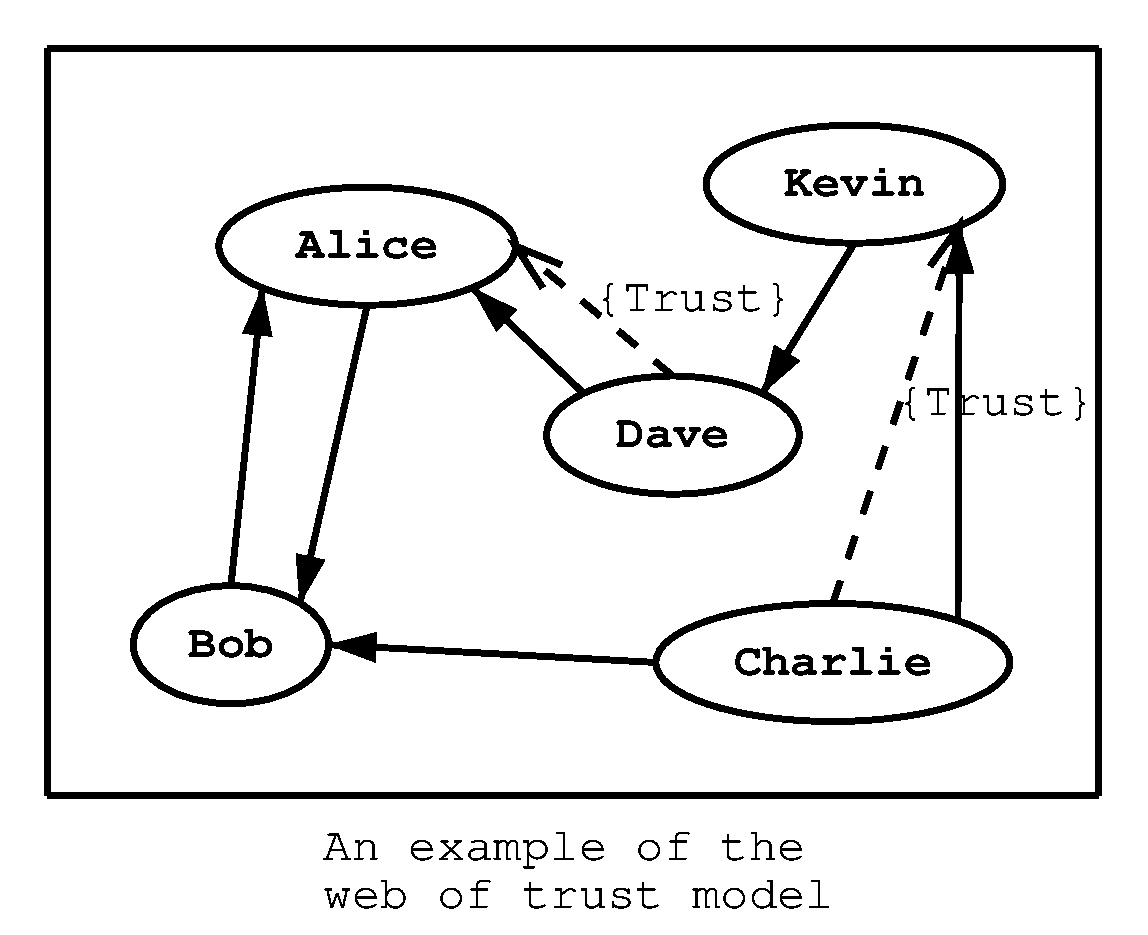
\includegraphics[height=9cm,width=11cm]{pgp-fig1}
\label{fig:pgp1}
\end{figure}

For example: If David trusts Alice to be an introducer, and Alice signed
Bob's key, Dave also trusts Bob's key to be the real one.

There are some key points that are important in that model. In the example
Alice has to sign Bob's key, only if she is sure that the key belongs
to Bob. Otherwise she may also make Dave falsely believe that this
is Bob's key. Dave has also the responsibility to know who to trust.
This model is similar to real life relations.

Just see how Charlie behaves in the previous example. Although he has 
signed Bob's key - because he knows, somehow, that it belongs to Bob - 
he does not trust Bob to be an introducer. Charlie decided to trust only 
Kevin, for some reason. A reason could be that Bob is lazy enough, and 
signs other people's keys without being sure that they belong to the 
actual owner.

\subsection*{OpenPGP keys}
In \gnutls{} the OpenPGP key structures \cite{RFC2440} are handled using the
\emph{gnutls\_openpgp\_key} type and the corresponding private keys with
the \emph{gnutls\_openpgp\_privkey} type. All the prototypes for the key handling
functions can be found at \emph{gnutls/openpgp.h}.

\subsection*{Verifying an OpenPGP key}
The verification functions of OpenPGP keys, included in \gnutls{}, 
are simple ones, and do not use the features of the ``web of trust''.
For that reason, if the verification needs are complex, 
the assistance of external tools like GnuPG is recommended.
\par
There are two verification functions in \gnutls{},
The \printfunc{gnutls_openpgp_key_verify_ring}{gnutls\_openpgp\_key\_verify\_ring}
and the \printfunc{gnutls_openpgp_key_verify_trustdb}{gnutls\_openpgp\_key\_verify\_trustdb}. 
The first one checks an OpenPGP key against a given set of public keys (keyring) and
returns the key status. The key verification status is the same as in X.509 certificates,
although the meaning and interpretation are different. For example an OpenPGP key may
be valid, if the self signature is ok, even if no signers were found.
The meaning of verification status is shown in figure \ref{fig:pgp_verify}.
\\
The latter function checks a GnuPG trust database for the given key. This function does not
check the key signatures, only checks for disabled and revoked keys.

\begin{figure}[hbtp]
\begin{tabular}{|l|p{7cm}|}

\hline
CERT\_INVALID & A signature on the key is invalid. That means that the key was modified
by somebody, or corrupted during transport.
\\
\hline
CERT\_REVOKED & The key has been revoked by its owner.
\\
\hline
CERT\_SIGNER\_NOT\_FOUND & The key was not signed by a known signer.
\\
\hline
\end{tabular}
\caption{OpenPGP key verification}
\label{fig:pgp_verify}
\end{figure}

